\documentclass{article}

% content/resources/templates/preamble.tex
\usepackage[margin=0.6in]{geometry}
\author{Milav Dabgar}
\usepackage{amsmath,amssymb,amsthm}
\usepackage{booktabs}
\usepackage{multirow}
\usepackage{xcolor}
\usepackage{tcolorbox}
\tcbuselibrary{breakable,skins}
\usepackage[colorlinks=true,linkcolor=blue]{hyperref}
\usepackage{titlesec}
\usepackage{enumitem}
\usepackage{tikz}
\usepackage{pgfplots}
\usepackage{circuitikz}
\usepackage[version=4]{mhchem}
\usepackage{longtable}
\usepackage{array}
\usepackage{float}
\usepackage{caption}
\usepackage{listings}

\lstset{
  basicstyle=\small\ttfamily,
  breaklines=true,
  breakatwhitespace=false,
  postbreak=\mbox{\textcolor{red}{$\hookrightarrow$}\space},
  float=false,
  numbers=left,
  numberstyle=\tiny\color{gray},
  numbersep=10pt,
  xleftmargin=2em,
  keywordstyle=\color{blue},
  commentstyle=\color{green!60!black},
  stringstyle=\color{purple},
  backgroundcolor=\color{gray!5},
  showstringspaces=false,
  tabsize=2,
  captionpos=b,
  keepspaces=true,
  columns=flexible
}

\pgfplotsset{compat=1.18}
\usetikzlibrary{shapes,arrows,positioning,calc,patterns,decorations.pathmorphing,decorations.markings,arrows.meta}

% Color scheme
\definecolor{headcolor}{RGB}{0,102,204}
\definecolor{keycolor}{RGB}{220,20,60}
\definecolor{solutioncolor}{RGB}{34,139,34}
\definecolor{mnemoniccolor}{RGB}{148,0,211}
\definecolor{codecolor}{RGB}{0,0,100}

% Spacing
\setlength{\parskip}{3pt}
\setlist[itemize]{nosep}
\setlist[enumerate]{nosep}

% Title formatting
\titleformat{\section}{\Large\bfseries\color{headcolor}}{\thesection}{1em}{}
\titleformat{\subsection}{\large\bfseries\color{headcolor}}{\thesubsection}{1em}{}

% Pandoc tightlist compatibility
\providecommand{\tightlist}{%
  \setlength{\itemsep}{0pt}\setlength{\parskip}{0pt}}

% Pandoc longtable compatibility
\newcounter{none}
\def\thenone{}


% content/resources/templates/english-boxes.tex

% Custom environments
\newtcolorbox{solutionbox}{
 breakable,
 enhanced,
 colback=solutioncolor!5!white,
 colframe=solutioncolor!75!black,
 fonttitle=\bfseries,
 title=Solution
}

\newtcolorbox{solutionboxnobreak}{
 colback=solutioncolor!5!white,
 colframe=solutioncolor!75!black,
 fonttitle=\bfseries,
 title=Solution
}

\newtcolorbox{keyformula}{
 breakable,
 enhanced,
 colback=keycolor!5!white,
 colframe=keycolor!75!black,
 fonttitle=\bfseries,
 title=Key Formula
}

\newtcolorbox{mnemonicboxenv}{
 breakable,
 enhanced,
 colback=mnemoniccolor!5!white,
 colframe=mnemoniccolor!75!black,
 fonttitle=\bfseries,
 title=Mnemonic
}

\newcommand{\mnemonicbox}[1]{%
  \begin{mnemonicboxenv}
    #1
  \end{mnemonicboxenv}
}


% Custom commands for GTU solutions
% This file defines semantic commands for consistent formatting

% Question command with automatic formatting
\newcommand{\question}[2]{%
  \section*{Question #1}%
  \textbf{#2}%
}

% OR question variant
\newcommand{\questionor}[2]{%
  \section*{Question #1 OR}%
  \textbf{#2}%
}

% Proper table environment with caption
\newenvironment{answertable}[1]{%
  \begin{table}[htbp]
  \centering
  \caption{#1}
}{%
  \end{table}
}

% Proper figure environment for diagrams
\newenvironment{answerdiagram}[1]{%
  \begin{figure}[htbp]
  \centering
  \caption{#1}
}{%
  \end{figure}
}

% Semantic markup for key terms
\newcommand{\keyword}[1]{\textbf{#1}}
\newcommand{\code}[1]{\texttt{#1}}
\newcommand{\classname}[1]{\texttt{#1}}
\newcommand{\methodname}[1]{\texttt{#1}}

% Proper quotation marks
\newcommand{\mnemonic}[1]{``#1''}


\title{Environment and Sustainability (4300003) - Winter 2023 Solution}
\date{January 11, 2024}

\begin{document}
\maketitle

\questionmarks{1(a)}{3}{Explain ecological footprint.}

\begin{solutionbox}
Ecological footprint measures the demand on nature by individuals, communities, or nations in terms of biologically productive land and water area required to sustain their lifestyle.

\begin{center}
\captionof{table}{Components of Ecological Footprint}
\begin{tabulary}{\linewidth}{|L|L|}
\hline
\textbf{Component} & \textbf{Description} \\ \hline
\textbf{Carbon Footprint} & Land needed to absorb CO\textsubscript{2} emissions \\ \hline
\textbf{Cropland} & Area for food production \\ \hline
\textbf{Grazing Land} & Area for livestock \\ \hline
\textbf{Forest Products} & Area for timber and paper \\ \hline
\textbf{Built-up Land} & Infrastructure and urban areas \\ \hline
\end{tabulary}
\end{center}

\begin{itemize}
    \item \keyword{Global hectares}: Standard unit for measurement
    \item \keyword{Overshoot}: When footprint exceeds biocapacity
    \item \keyword{Sustainability}: Balance between consumption and regeneration
\end{itemize}
\end{solutionbox}

\begin{mnemonicbox}
\mnemonic{CGFBB: Carbon, Cropland, Grazing, Forest, Built-up}
\end{mnemonicbox}

\questionmarks{1(b)}{4}{Explain Eltonian pyramid.}

\begin{solutionbox}
Eltonian pyramid (Pyramid of Numbers) shows the number of organisms at each trophic level in an ecosystem, proposed by Charles Elton.

\begin{center}
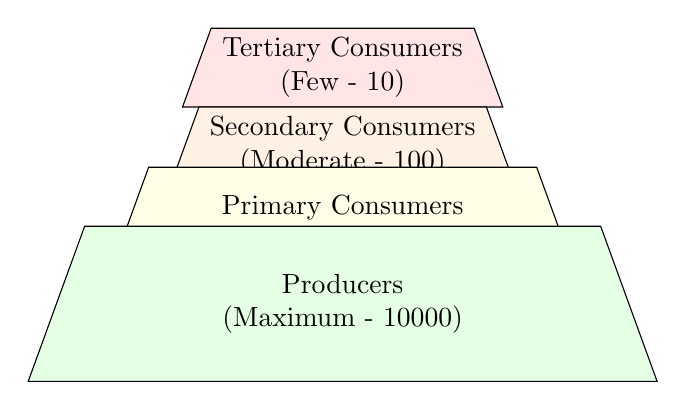
\begin{tikzpicture}[node distance=0cm, outer sep=0pt]
    \node [draw, trapezium, trapezium angle=70, minimum width=2cm, minimum height=1cm, fill=red!10, align=center] (T) at (0,3) {Tertiary Consumers\\(Few - 10)};
    \node [draw, trapezium, trapezium angle=70, minimum width=4cm, minimum height=1cm, fill=orange!10, align=center] (S) at (0,2) {Secondary Consumers\\(Moderate - 100)};
    \node [draw, trapezium, trapezium angle=70, minimum width=6cm, minimum height=1cm, fill=yellow!10, align=center] (P) at (0,1) {Primary Consumers\\(Many - 1000)};
    \node [draw, trapezium, trapezium angle=70, minimum width=8cm, minimum height=1cm, fill=green!10, align=center] (Pr) at (0,0) {Producers\\(Maximum - 10000)};
\end{tikzpicture}
\captionof{figure}{Eltonian Pyramid of Numbers}
\end{center}

\begin{center}
\captionof{table}{Pyramid Types}
\begin{tabulary}{\linewidth}{|L|L|L|}
\hline
\textbf{Type} & \textbf{Basis} & \textbf{Shape} \\ \hline
\textbf{Numbers} & Individual count & Usually upright \\ \hline
\textbf{Biomass} & Total weight & Can be inverted \\ \hline
\textbf{Energy} & Energy flow & Always upright \\ \hline
\end{tabulary}
\end{center}

\begin{itemize}
    \item \keyword{Trophic levels}: Feeding positions in food chain
    \item \keyword{10\% rule}: Only 10\% energy transfers to next level
    \item \keyword{Exceptions}: Tree ecosystem shows inverted number pyramid
\end{itemize}
\end{solutionbox}

\begin{mnemonicbox}
\mnemonic{ELTON: Energy Loss Through Organism Numbers}
\end{mnemonicbox}

\questionmarks{1(c)}{7}{Explain Eco-system with its classification and component.}

\begin{solutionbox}
Ecosystem is a functional unit of nature where living organisms interact with each other and their physical environment, involving energy flow and nutrient cycling.

\begin{center}
\captionof{table}{Ecosystem Components}
\begin{tabulary}{\linewidth}{|L|L|L|}
\hline
\textbf{Component} & \textbf{Type} & \textbf{Examples} \\ \hline
\textbf{Abiotic} & Non-living & Air, water, soil, climate \\ \hline
\textbf{Biotic} & Living & Plants, animals, microorganisms \\ \hline
\textbf{Producers} & Autotrophs & Green plants, algae \\ \hline
\textbf{Consumers} & Heterotrophs & Herbivores, carnivores, omnivores \\ \hline
\textbf{Decomposers} & Recyclers & Bacteria, fungi \\ \hline
\end{tabulary}
\end{center}

\textbf{Classification of Ecosystems:}

\textbf{Natural Ecosystems:}
\begin{itemize}
    \item \keyword{Terrestrial}: Forest, grassland, desert
    \item \keyword{Aquatic}: Freshwater (pond, river), Marine (ocean, sea)
\end{itemize}

\textbf{Artificial Ecosystems:}
\begin{itemize}
    \item \keyword{Agricultural}: Crop fields, gardens
    \item \keyword{Urban}: Parks, artificial lakes
\end{itemize}

\begin{center}
\begin{tikzpicture}[node distance=1.5cm, auto]
    \node [gtu block] (Sun) {Sun};
    \node [gtu block, right=1.5cm of Sun] (Prod) {Producers};
    \node [gtu block, right=1.5cm of Prod] (PC) {Primary\\Consumers};
    \node [gtu block, right=1.5cm of PC] (SC) {Secondary\\Consumers};
    \node [gtu block, right=1.5cm of SC] (TC) {Tertiary\\Consumers};
    \node [gtu block, below=1.5cm of PC] (Dec) {Decomposers};

    \path [gtu arrow] (Sun) -- (Prod);
    \path [gtu arrow] (Prod) -- (PC);
    \path [gtu arrow] (PC) -- (SC);
    \path [gtu arrow] (SC) -- (TC);
    \path [gtu arrow] (Prod) -- (Dec);
    \path [gtu arrow] (PC) -- (Dec);
    \path [gtu arrow] (SC) -- (Dec);
    \path [gtu arrow] (TC) -- (Dec);
    \path [gtu arrow] (Dec) -| (Prod);
\end{tikzpicture}
\captionof{figure}{Energy Flow in Ecosystem}
\end{center}

\begin{itemize}
    \item \keyword{Energy flow}: Unidirectional from sun to decomposers
    \item \keyword{Nutrient cycling}: Cyclical movement of elements
    \item \keyword{Food chains}: Linear energy transfer
    \item \keyword{Food webs}: Interconnected food chains
\end{itemize}
\end{solutionbox}

\begin{mnemonicbox}
\mnemonic{PEACE: Producers, Energy, Animals, Cycles, Environment}
\end{mnemonicbox}

\questionmarks{1(c OR)}{7}{Explain Nitrogen cycle.}

\begin{solutionbox}
Nitrogen cycle is the biogeochemical cycle that converts nitrogen compounds through various chemical forms as it circulates through atmosphere, terrestrial and aquatic systems.

\begin{center}
\begin{tikzpicture}[node distance=2cm, auto]
    \node [gtu block] (N2) {Atmospheric N\textsubscript{2}};
    \node [gtu block, below right=2cm of N2] (NH3) {Ammonia NH\textsubscript{3}};
    \node [gtu block, below=1.5cm of NH3] (NO2) {Nitrites NO\textsubscript{2}\textsuperscript{-}};
    \node [gtu block, left=2cm of NO2] (NO3) {Nitrates NO\textsubscript{3}\textsuperscript{-}};
    \node [gtu block, above left=1.5cm of NO3] (Bio) {Plant \& Animal\\Biomass};
    
    % Fixation
    \path [gtu arrow] (N2) -- node[midway, right] {Fixation} (NH3);
    % Nitrification
    \path [gtu arrow] (NH3) -- node[midway, right] {Nitrification} (NO2);
    \path [gtu arrow] (NO2) -- (NO3);
    % Assimilation
    \path [gtu arrow] (NO3) -- node[midway, left] {Assimilation} (Bio);
    % Decomposition
    \path [gtu arrow] (Bio) -- node[midway, above] {Decomposition} (NH3);
    % Denitrification
    \path [gtu arrow] (NO3) -- node[midway, left] {Denitrification} (N2);
\end{tikzpicture}
\captionof{figure}{Nitrogen Cycle}
\end{center}

\begin{center}
\captionof{table}{Nitrogen Cycle Processes}
\begin{tabulary}{\linewidth}{|L|L|L|}
\hline
\textbf{Process} & \textbf{Conversion} & \textbf{Organisms} \\ \hline
\textbf{Fixation} & N\textsubscript{2} $\rightarrow$ NH\textsubscript{3} & Rhizobium, Azotobacter \\ \hline
\textbf{Nitrification} & NH\textsubscript{3} $\rightarrow$ NO\textsubscript{2}\textsuperscript{-} $\rightarrow$ NO\textsubscript{3}\textsuperscript{-} & Nitrosomonas, Nitrobacter \\ \hline
\textbf{Assimilation} & NO\textsubscript{3}\textsuperscript{-} $\rightarrow$ Proteins & Plants \\ \hline
\textbf{Decomposition} & Proteins $\rightarrow$ NH\textsubscript{3} & Bacteria, fungi \\ \hline
\textbf{Denitrification} & NO\textsubscript{3}\textsuperscript{-} $\rightarrow$ N\textsubscript{2} & Anaerobic bacteria \\ \hline
\end{tabulary}
\end{center}

\begin{itemize}
    \item \keyword{Biological fixation}: 80\% of total fixation
    \item \keyword{Industrial fixation}: Haber process for fertilizers
    \item \keyword{Lightning}: Natural atmospheric fixation
    \item \keyword{Pollution}: Excess nitrates cause eutrophication
\end{itemize}
\end{solutionbox}

\begin{mnemonicbox}
\mnemonic{FNADD: Fixation, Nitrification, Assimilation, Decomposition, Denitrification}
\end{mnemonicbox}

\questionmarks{2(a)}{3}{List the waste water quality parameter.}

\begin{solutionbox}
\begin{center}
\captionof{table}{Wastewater Quality Parameters}
\begin{tabulary}{\linewidth}{|L|L|L|}
\hline
\textbf{Physical} & \textbf{Chemical} & \textbf{Biological} \\ \hline
\textbf{Turbidity} & \textbf{BOD} & \textbf{Coliform count} \\ \hline
\textbf{Color} & \textbf{COD} & \textbf{Pathogenic bacteria} \\ \hline
\textbf{Odor} & \textbf{pH} & \textbf{Algae} \\ \hline
\textbf{Temperature} & \textbf{DO} & \textbf{Virus} \\ \hline
\textbf{Total Solids} & \textbf{Ammonia} & \textbf{Protozoa} \\ \hline
\end{tabulary}
\end{center}

\begin{itemize}
    \item \keyword{Primary parameters}: BOD, COD, pH, suspended solids
    \item \keyword{Secondary parameters}: Heavy metals, nutrients
    \item \keyword{Indicator organisms}: \textit{E.coli} for fecal contamination
\end{itemize}
\end{solutionbox}

\begin{mnemonicbox}
\mnemonic{PCB: Physical, Chemical, Biological parameters}
\end{mnemonicbox}

\questionmarks{2(b)}{4}{Explain E-waste classification and effects.}

\begin{solutionbox}
Electronic waste (E-waste) refers to discarded electrical and electronic equipment containing hazardous materials.

\begin{center}
\captionof{table}{E-waste Classification}
\begin{tabulary}{\linewidth}{|L|L|L|}
\hline
\textbf{Category} & \textbf{Examples} & \textbf{Hazardous Materials} \\ \hline
\textbf{Large Appliances} & Refrigerators, washing machines & CFCs, heavy metals \\ \hline
\textbf{Small Appliances} & Microwaves, toasters & Lead, mercury \\ \hline
\textbf{IT Equipment} & Computers, printers & Cadmium, chromium \\ \hline
\textbf{Telecom Equipment} & Mobile phones, cables & Beryllium, flame retardants \\ \hline
\textbf{Consumer Electronics} & TVs, radios & Polyvinyl chloride (PVC) \\ \hline
\end{tabulary}
\end{center}

\textbf{Effects of E-waste:}
\begin{itemize}
    \item \keyword{Environmental}: Soil and water pollution, air contamination
    \item \keyword{Health}: Cancer, neurological disorders, respiratory problems
    \item \keyword{Resource depletion}: Loss of valuable metals like gold, silver
    \item \keyword{Ecosystem damage}: Bioaccumulation in food chain
\end{itemize}
\end{solutionbox}

\begin{mnemonicbox}
\mnemonic{LSITC: Large, Small, IT, Telecom, Consumer electronics}
\end{mnemonicbox}

\questionmarks{2(c)}{7}{Explain Electrostatic precipitators.}

\begin{solutionbox}
Electrostatic precipitators (ESP) are air pollution control devices that remove particulate matter from industrial gas streams using electrical charges.

\begin{center}
\begin{tikzpicture}[node distance=1cm, auto]
    \node [gtu block, minimum width=6cm, minimum height=3cm] (Box) {};
    \node [left=1cm of Box.west] (In) {Dirty Gas Input};
    \node [right=1cm of Box.east] (Out) {Clean Gas Output};
    
    \node [draw, circle, fill=black, inner sep=1pt] (Elec1) at (Box.center) {};
    \node [above=0.2cm of Elec1] {+ Electrode};
    
    \draw [thick] (Box.north west) -- (Box.north east);
    \draw [thick] (Box.south west) -- (Box.south east);
    
    \node [above=0.1cm of Box.south] {- Collection Plate};
    
    \node [draw, trapezium, trapezium angle=60, shape border rotate=180, minimum width=2cm, below=0cm of Box] (Hopper) {Dust Collection Hopper};
    
    \draw [gtu arrow] (In) -- (Box.west);
    \draw [gtu arrow] (Box.east) -- (Out);
\end{tikzpicture}
\captionof{figure}{ESP Working Principle}
\end{center}

\begin{center}
\captionof{table}{ESP Components and Functions}
\begin{tabulary}{\linewidth}{|L|L|L|}
\hline
\textbf{Component} & \textbf{Function} & \textbf{Material} \\ \hline
\textbf{Discharge Electrode} & Creates corona discharge & Tungsten wire \\ \hline
\textbf{Collection Plate} & Attracts charged particles & Steel plates \\ \hline
\textbf{High Voltage Supply} & Provides 30-100 kV DC & Transformer-rectifier \\ \hline
\textbf{Rapper System} & Removes collected dust & Mechanical vibrator \\ \hline
\textbf{Hopper} & Collects fallen particles & Steel container \\ \hline
\end{tabulary}
\end{center}

\textbf{Working Principle:}
\begin{enumerate}
    \item \keyword{Ionization}: High voltage creates corona discharge
    \item \keyword{Charging}: Particles acquire negative charge
    \item \keyword{Collection}: Charged particles move to positive plates
    \item \keyword{Removal}: Rapping dislodges collected dust
\end{enumerate}

\textbf{Applications:}
\begin{itemize}
    \item \keyword{Power plants}: Coal-fired boilers
    \item \keyword{Cement industry}: Kiln gas cleaning
    \item \keyword{Steel industry}: Blast furnace gas
    \item \keyword{Chemical plants}: Process gas treatment
\end{itemize}

\textbf{Advantages:}
\begin{itemize}
    \item \keyword{High efficiency}: 99\%+ removal for fine particles
    \item \keyword{Low pressure drop}: Energy efficient operation
    \item \keyword{Handles high temperatures}: Up to 400\textdegree C
\end{itemize}
\end{solutionbox}

\begin{mnemonicbox}
\mnemonic{CHARGE: Corona, High-voltage, Attract, Rapper, Gas, Efficiency}
\end{mnemonicbox}

\questionmarks{2(a OR)}{3}{Explain (1) BOD (2) COD}

\begin{solutionbox}
\begin{center}
\captionof{table}{BOD vs COD}
\begin{tabulary}{\linewidth}{|L|L|L|}
\hline
\textbf{Parameter} & \textbf{BOD} & \textbf{COD} \\ \hline
\textbf{Full Form} & Biochemical Oxygen Demand & Chemical Oxygen Demand \\ \hline
\textbf{Method} & Biological oxidation & Chemical oxidation \\ \hline
\textbf{Time} & 5 days at 20\textdegree C & 2-3 hours \\ \hline
\textbf{Oxidizing Agent} & Microorganisms & Potassium dichromate \\ \hline
\end{tabulary}
\end{center}

\textbf{(1) BOD (Biochemical Oxygen Demand):}
\begin{itemize}
    \item \keyword{Definition}: Oxygen required by microorganisms to decompose organic matter
    \item \keyword{Standard conditions}: 5 days, 20\textdegree C, dark conditions
    \item \keyword{Units}: mg/L or ppm
\end{itemize}

\textbf{(2) COD (Chemical Oxygen Demand):}
\begin{itemize}
    \item \keyword{Definition}: Oxygen equivalent to oxidize organic matter chemically
    \item \keyword{Oxidizing agent}: K\textsubscript{2}Cr\textsubscript{2}O\textsubscript{7} in acidic medium
    \item \keyword{Higher than BOD}: Includes non-biodegradable compounds
\end{itemize}
\end{solutionbox}

\begin{mnemonicbox}
\mnemonic{BTCO: Biological Time, Chemical Oxidation}
\end{mnemonicbox}

\questionmarks{2(b OR)}{4}{Explain Recycle of E waste.}

\begin{solutionbox}
E-waste recycling is the process of recovering valuable materials from electronic waste while safely disposing of hazardous substances.

\begin{center}
\captionof{table}{E-waste Recycling Process}
\begin{tabulary}{\linewidth}{|L|L|L|}
\hline
\textbf{Stage} & \textbf{Process} & \textbf{Recovery} \\ \hline
\textbf{Collection} & Gathering from households, offices & Whole devices \\ \hline
\textbf{Dismantling} & Manual separation of components & Plastics, metals, circuit boards \\ \hline
\textbf{Shredding} & Mechanical size reduction & Mixed material streams \\ \hline
\textbf{Separation} & Magnetic, density, optical sorting & Ferrous, non-ferrous metals \\ \hline
\textbf{Refining} & Chemical processing & Pure metals (Au, Ag, Cu, Pd) \\ \hline
\end{tabulary}
\end{center}

\textbf{Recycling Methods:}
\begin{itemize}
    \item \keyword{Mechanical}: Physical separation and size reduction
    \item \keyword{Pyrometallurgy}: High-temperature metal recovery
    \item \keyword{Hydrometallurgy}: Chemical leaching processes
    \item \keyword{Biotechnology}: Microbial metal extraction
\end{itemize}

\textbf{Benefits:}
\begin{itemize}
    \item \keyword{Resource conservation}: Recovery of precious metals
    \item \keyword{Environmental protection}: Prevents soil and water contamination
    \item \keyword{Economic value}: Job creation and revenue generation
    \item \keyword{Energy savings}: Less energy than primary production
\end{itemize}
\end{solutionbox}

\begin{mnemonicbox}
\mnemonic{CDSPR: Collection, Dismantling, Shredding, Separation, Refining}
\end{mnemonicbox}

\questionmarks{2(c OR)}{7}{Define pollution and its source. Explain the classification of pollutants.}

\begin{solutionbox}
\textbf{Definition:} Pollution is the introduction of harmful substances or energy into the environment, causing adverse changes to air, water, soil, or living organisms.

\begin{center}
\captionof{table}{Sources of Pollution}
\begin{tabulary}{\linewidth}{|L|L|L|}
\hline
\textbf{Source Type} & \textbf{Examples} & \textbf{Pollutants Released} \\ \hline
\textbf{Point Sources} & Industrial chimneys, sewage outfalls & Specific location discharge \\ \hline
\textbf{Non-point Sources} & Agricultural runoff, urban stormwater & Diffuse area pollution \\ \hline
\textbf{Mobile Sources} & Vehicles, ships, aircraft & Exhaust emissions \\ \hline
\textbf{Stationary Sources} & Power plants, factories & Stack emissions \\ \hline
\end{tabulary}
\end{center}

\textbf{Classification of Pollutants:}

\textbf{1. By Nature:}
\begin{center}
\captionof{table}{Pollutant Classification by Nature}
\begin{tabulary}{\linewidth}{|L|L|L|}
\hline
\textbf{Type} & \textbf{Characteristics} & \textbf{Examples} \\ \hline
\textbf{Biodegradable} & Decompose naturally & Organic waste, sewage \\ \hline
\textbf{Non-biodegradable} & Persist in environment & Plastics, heavy metals \\ \hline
\textbf{Slowly degradable} & Decompose over years & Pesticides, radioactive materials \\ \hline
\end{tabulary}
\end{center}

\textbf{2. By Form:}
\begin{itemize}
    \item \keyword{Primary}: Directly emitted (SO\textsubscript{2}, CO, particulates)
    \item \keyword{Secondary}: Formed by reactions (O\textsubscript{3}, acid rain, smog)
\end{itemize}

\textbf{3. By Source:}
\begin{itemize}
    \item \keyword{Natural}: Volcanic eruptions, forest fires
    \item \keyword{Anthropogenic}: Human activities, industrial processes
\end{itemize}

\begin{center}
\begin{tikzpicture}[node distance=1.5cm, auto]
    \node [gtu block] (P) {Pollutants};
    \node [gtu block, below left=1.5cm of P] (N) {By Nature};
    \node [gtu block, below=1.5cm of P] (F) {By Form};
    \node [gtu block, below right=1.5cm of P] (S) {By Source};
    
    \node [gtu block, below left=0.5cm of N] (Bio) {Biodegradable};
    \node [gtu block, below right=0.5cm of N] (Non) {Non-biodegradable};
    
    \node [gtu block, below left=0.5cm of F] (Pri) {Primary};
    \node [gtu block, below right=0.5cm of F] (Sec) {Secondary};
    
    \node [gtu block, below left=0.5cm of S] (Nat) {Natural};
    \node [gtu block, below right=0.5cm of S] (Anth) {Anthropogenic};
    
    \path [gtu arrow] (P) -- (N);
    \path [gtu arrow] (P) -- (F);
    \path [gtu arrow] (P) -- (S);
    
    \path [gtu arrow] (N) -- (Bio);
    \path [gtu arrow] (N) -- (Non);
    \path [gtu arrow] (F) -- (Pri);
    \path [gtu arrow] (F) -- (Sec);
    \path [gtu arrow] (S) -- (Nat);
    \path [gtu arrow] (S) -- (Anth);
\end{tikzpicture}
\captionof{figure}{Pollution Classification}
\end{center}

\textbf{Effects of Pollution:}
\begin{itemize}
    \item \keyword{Environmental}: Ecosystem disruption, species extinction
    \item \keyword{Health}: Respiratory diseases, cancer, genetic disorders
    \item \keyword{Economic}: Healthcare costs, reduced productivity
    \item \keyword{Social}: Quality of life degradation
\end{itemize}
\end{solutionbox}

\begin{mnemonicbox}
\mnemonic{BNS-PFC: Biodegradable, Non-biodegradable, Slowly degradable - Primary, Form, Classification}
\end{mnemonicbox}


\questionmarks{3(a)}{3}{State the working of solar cell.}

\begin{solutionbox}
Solar cell converts light energy directly into electrical energy through photovoltaic effect using semiconductor materials.

\begin{center}
\captionof{table}{Solar Cell Working Process}
\begin{tabulary}{\linewidth}{|L|L|L|}
\hline
\textbf{Step} & \textbf{Process} & \textbf{Result} \\ \hline
\textbf{Photon Absorption} & Light hits semiconductor & Electron excitation \\ \hline
\textbf{Electron-Hole Generation} & Energy breaks bonds & Free charge carriers \\ \hline
\textbf{Charge Separation} & Built-in electric field & Electrons to n-side, holes to p-side \\ \hline
\textbf{Current Collection} & External circuit connection & Electrical current flow \\ \hline
\end{tabulary}
\end{center}

\begin{itemize}
    \item \keyword{p-n junction}: Creates internal electric field
    \item \keyword{Depletion region}: Area with charge separation
    \item \keyword{External load}: Completes electrical circuit
\end{itemize}
\end{solutionbox}

\begin{mnemonicbox}
\mnemonic{PECS: Photon, Electron, Charge, Separation}
\end{mnemonicbox}

\questionmarks{3(b)}{4}{Give the comparison between Horizontal Axis and Vertical Axis wind mills.}

\begin{solutionbox}
\begin{center}
\captionof{table}{HAWT vs VAWT Comparison}
\begin{tabulary}{\linewidth}{|L|L|L|}
\hline
\textbf{Parameter} & \textbf{Horizontal Axis (HAWT)} & \textbf{Vertical Axis (VAWT)} \\ \hline
\textbf{Blade Orientation} & Horizontal rotation & Vertical rotation \\ \hline
\textbf{Wind Direction} & Must face wind & Accepts from any direction \\ \hline
\textbf{Efficiency} & Higher (35-45\%) & Lower (20-35\%) \\ \hline
\textbf{Height} & Tower mounted, high & Ground level installation \\ \hline
\textbf{Maintenance} & Difficult, high altitude & Easy, ground accessible \\ \hline
\textbf{Noise} & Moderate & Lower \\ \hline
\textbf{Cost} & Higher initial & Lower installation \\ \hline
\textbf{Power Output} & Higher for large scale & Suitable for small scale \\ \hline
\end{tabulary}
\end{center}

\textbf{Advantages:}
\begin{itemize}
    \item \keyword{HAWT}: Higher efficiency, proven technology, better power-to-weight ratio
    \item \keyword{VAWT}: Omnidirectional, easier maintenance, quieter operation, urban friendly
\end{itemize}

\textbf{Applications:}
\begin{itemize}
    \item \keyword{HAWT}: Large wind farms, utility-scale power generation
    \item \keyword{VAWT}: Urban areas, small-scale applications, distributed generation
\end{itemize}
\end{solutionbox}

\begin{mnemonicbox}
\mnemonic{HEAVEN: Height, Efficiency, Accessibility, Versatility, Economics, Noise}
\end{mnemonicbox}

\questionmarks{3(c)}{7}{Explain construction and working of Biogas plant with sketch.}

\begin{solutionbox}
Biogas plant produces methane-rich gas through anaerobic digestion of organic waste materials by methanogenic bacteria.

\begin{center}
\begin{tikzpicture}[node distance=1.5cm, auto]
    \node [gtu block, minimum width=3cm, minimum height=2cm] (Digester) {Digester};
    \node [gtu block, above=1cm of Digester] (GasHolder) {Gas Holder};
    \node [left=1.5cm of Digester] (Inlet) {Feed Inlet};
    \node [right=1.5cm of Digester] (Outlet) {Slurry Outlet};
    \node [above=1cm of GasHolder] (GasOut) {Gas Outlet};
    
    \node [draw, dashed, fit=(Digester) (GasHolder), label=below:Underground Chamber] (Chamber) {};
    
    \path [gtu arrow] (Inlet) -- (Digester);
    \path [gtu arrow] (Digester) -- (Outlet);
    \path [gtu arrow] (Digester) -- (GasHolder);
    \path [gtu arrow] (GasHolder) -- (GasOut);
\end{tikzpicture}
\captionof{figure}{Biogas Plant Schematic}
\end{center}

\begin{center}
\captionof{table}{Biogas Plant Components}
\begin{tabulary}{\linewidth}{|L|L|L|}
\hline
\textbf{Component} & \textbf{Function} & \textbf{Material} \\ \hline
\textbf{Digester} & Anaerobic fermentation chamber & Concrete/steel \\ \hline
\textbf{Gas Holder} & Gas storage and pressure regulation & Steel/plastic \\ \hline
\textbf{Inlet Chamber} & Feed material entry & Masonry \\ \hline
\textbf{Outlet Chamber} & Slurry discharge & Masonry \\ \hline
\textbf{Mixing Tank} & Raw material preparation & Concrete \\ \hline
\end{tabulary}
\end{center}

\textbf{Construction Details:}

\textbf{Underground Digester:}
\begin{itemize}
    \item \keyword{Shape}: Cylindrical or dome-shaped
    \item \keyword{Capacity}: 10-100 m\textsuperscript{3} for household plants
    \item \keyword{Wall thickness}: 10-15 cm concrete
    \item \keyword{Insulation}: Prevents heat loss
\end{itemize}

\textbf{Working Process:}

\begin{center}
\captionof{table}{Biogas Production Stages}
\begin{tabulary}{\linewidth}{|L|L|L|L|}
\hline
\textbf{Stage} & \textbf{Process} & \textbf{Duration} & \textbf{Products} \\ \hline
\textbf{Hydrolysis} & Large molecules breakdown & 1-3 days & Simple sugars, amino acids \\ \hline
\textbf{Acidogenesis} & Acid formation & 3-7 days & Organic acids, alcohols \\ \hline
\textbf{Methanogenesis} & Methane production & 15-30 days & CH\textsubscript{4} (60\%), CO\textsubscript{2} (40\%) \\ \hline
\end{tabulary}
\end{center}

\textbf{Operating Conditions:}
\begin{itemize}
    \item \keyword{Temperature}: 30-40\textdegree C (mesophilic)
    \item \keyword{pH}: 6.8-7.2 (neutral)
    \item \keyword{C:N ratio}: 25-30:1 optimal
    \item \keyword{Retention time}: 20-30 days
\end{itemize}

\textbf{Applications:}
\begin{itemize}
    \item \keyword{Cooking}: Clean burning fuel
    \item \keyword{Lighting}: Gas lamps
    \item \keyword{Heating}: Space and water heating
    \item \keyword{Electricity}: Generator sets
\end{itemize}

\textbf{Advantages:}
\begin{itemize}
    \item \keyword{Renewable energy}: Sustainable fuel source
    \item \keyword{Waste management}: Organic waste disposal
    \item \keyword{Fertilizer production}: Nutrient-rich slurry
    \item \keyword{Environmental benefits}: Reduces greenhouse gases
\end{itemize}
\end{solutionbox}

\begin{mnemonicbox}
\mnemonic{BIGHM: Biological, Input, Gas, Holder, Methane}
\end{mnemonicbox}

\questionmarks{3(a OR)}{3}{List the advantages of flat plate collector.}

\begin{solutionbox}
\begin{center}
\captionof{table}{Flat Plate Collector Advantages}
\begin{tabulary}{\linewidth}{|L|L|}
\hline
\textbf{Category} & \textbf{Advantages} \\ \hline
\textbf{Technical} & Simple design, no moving parts, low maintenance \\ \hline
\textbf{Economic} & Low cost, mass production possible \\ \hline
\textbf{Operational} & Works with diffuse light, handles both direct and indirect radiation \\ \hline
\textbf{Durability} & Long life (15-20 years), weather resistant \\ \hline
\textbf{Versatility} & Multiple applications, modular installation \\ \hline
\end{tabulary}
\end{center}

\textbf{Key Benefits:}
\begin{itemize}
    \item \keyword{Reliability}: No complex mechanisms or controls required
    \item \keyword{Efficiency}: 40-60\% thermal efficiency in optimal conditions
    \item \keyword{Installation}: Easy mounting on roofs or ground
\end{itemize}
\end{solutionbox}

\begin{mnemonicbox}
\mnemonic{TEODV: Technical, Economic, Operational, Durability, Versatility}
\end{mnemonicbox}

\questionmarks{3(b OR)}{4}{What is wind farm? List its advantages.}

\begin{solutionbox}
\textbf{Definition:} Wind farm is a group of wind turbines installed in the same location for commercial electricity generation, connected to electrical grid through transmission lines.

\begin{center}
\captionof{table}{Wind Farm Advantages}
\begin{tabulary}{\linewidth}{|L|L|}
\hline
\textbf{Category} & \textbf{Advantages} \\ \hline
\textbf{Environmental} & Clean energy, zero emissions, reduces carbon footprint \\ \hline
\textbf{Economic} & Job creation, low operating costs, revenue for landowners \\ \hline
\textbf{Technical} & Scalable capacity, grid stability, energy independence \\ \hline
\textbf{Social} & Rural development, community benefits, educational opportunities \\ \hline
\end{tabulary}
\end{center}

\textbf{Specific Benefits:}
\begin{itemize}
    \item \keyword{Land use efficiency}: Farming can continue between turbines
    \item \keyword{Quick installation}: Faster than conventional power plants
    \item \keyword{Predictable costs}: Fixed fuel cost (wind is free)
    \item \keyword{Modular expansion}: Capacity can be increased incrementally
\end{itemize}

\textbf{Applications:}
\begin{itemize}
    \item \keyword{Onshore}: Land-based installations
    \item \keyword{Offshore}: Ocean-based for higher wind speeds
    \item \keyword{Distributed}: Small-scale community projects
\end{itemize}
\end{solutionbox}

\begin{mnemonicbox}
\mnemonic{ECTS: Environmental, Economic, Technical, Social benefits}
\end{mnemonicbox}

\questionmarks{3(c OR)}{7}{Explain in brief (1) Geothermal energy (2) Tidal energy}

\begin{solutionbox}
\textbf{(1) Geothermal Energy:}

Geothermal energy harnesses heat from Earth's interior for electricity generation and direct heating applications.

\begin{center}
\captionof{table}{Geothermal Energy Systems}
\begin{tabulary}{\linewidth}{|L|L|L|}
\hline
\textbf{Type} & \textbf{Temperature} & \textbf{Applications} \\ \hline
\textbf{High Temperature} & >150\textdegree C & Electricity generation \\ \hline
\textbf{Medium Temperature} & 90-150\textdegree C & Direct heating, cooling \\ \hline
\textbf{Low Temperature} & <90\textdegree C & Heat pumps, agriculture \\ \hline
\end{tabulary}
\end{center}

\textbf{Working Principle:}
\begin{itemize}
    \item \keyword{Heat source}: Radioactive decay in Earth's core
    \item \keyword{Extraction}: Wells drilled to access hot water/steam
    \item \keyword{Conversion}: Steam drives turbines for electricity
    \item \keyword{Reinjection}: Water returned to reservoir
\end{itemize}

\textbf{(2) Tidal Energy:}

Tidal energy converts kinetic and potential energy of ocean tides into electricity using predictable tidal movements.

\begin{center}
\captionof{table}{Tidal Energy Technologies}
\begin{tabulary}{\linewidth}{|L|L|L|}
\hline
\textbf{Technology} & \textbf{Principle} & \textbf{Installation} \\ \hline
\textbf{Tidal Barrage} & Potential energy of tidal range & Dam across estuary \\ \hline
\textbf{Tidal Stream} & Kinetic energy of tidal currents & Underwater turbines \\ \hline
\textbf{Tidal Lagoon} & Artificial impoundment & Breakwater construction \\ \hline
\end{tabulary}
\end{center}

\textbf{Advantages:}
\begin{itemize}
    \item \keyword{Geothermal}: Baseload power, low emissions, small footprint, reliable
    \item \keyword{Tidal}: Predictable, high energy density, long lifespan, no fuel costs
\end{itemize}

\textbf{Challenges:}
\begin{itemize}
    \item \keyword{Geothermal}: Location specific, high initial cost, induced seismicity
    \item \keyword{Tidal}: High capital cost, environmental impact, limited locations
\end{itemize}
\end{solutionbox}

\begin{mnemonicbox}
\mnemonic{GT-POWER: Geothermal Temperature, Tidal Predictable Ocean Water Energy Resource}
\end{mnemonicbox}

\questionmarks{4(a)}{3}{Explain Need of Renewable energy.}

\begin{solutionbox}
\begin{center}
\captionof{table}{Need for Renewable Energy}
\begin{tabulary}{\linewidth}{|L|L|}
\hline
\textbf{Driver} & \textbf{Reasons} \\ \hline
\textbf{Environmental} & Climate change mitigation, reduced pollution \\ \hline
\textbf{Economic} & Energy security, price stability, job creation \\ \hline
\textbf{Technical} & Depleting fossil fuels, technological advancement \\ \hline
\textbf{Social} & Rural development, health benefits, energy access \\ \hline
\end{tabulary}
\end{center}

\textbf{Key Needs:}
\begin{itemize}
    \item \keyword{Climate commitments}: Meet Paris Agreement targets
    \item \keyword{Energy independence}: Reduce import dependence
    \item \keyword{Sustainable development}: Long-term energy security
\end{itemize}
\end{solutionbox}

\begin{mnemonicbox}
\mnemonic{EETS: Environmental, Economic, Technical, Social needs}
\end{mnemonicbox}

\questionmarks{4(b)}{4}{Explain Depletion of ozone layer.}

\begin{solutionbox}
Ozone layer depletion is the reduction of ozone concentration in stratosphere due to human-made chemicals, particularly chlorofluorocarbons (CFCs).

\begin{center}
\captionof{table}{Ozone Depletion Process}
\begin{tabulary}{\linewidth}{|L|L|L|}
\hline
\textbf{Stage} & \textbf{Process} & \textbf{Chemical Reaction} \\ \hline
\textbf{CFC Release} & Industrial emissions & CFCs rise to stratosphere \\ \hline
\textbf{UV Breakdown} & Photodissociation & CFC + UV $\rightarrow$ Cl + other products \\ \hline
\textbf{Ozone Destruction} & Catalytic cycle & Cl + O\textsubscript{3} $\rightarrow$ ClO + O\textsubscript{2} \\ \hline
\textbf{Chain Reaction} & Continuous process & ClO + O $\rightarrow$ Cl + O\textsubscript{2} \\ \hline
\end{tabulary}
\end{center}

\textbf{Causes:}
\begin{itemize}
    \item \keyword{Primary}: CFCs, halons, methyl bromide
    \item \keyword{Secondary}: HCFCs, nitrous oxide, carbon tetrachloride
\end{itemize}

\textbf{Effects:}
\begin{itemize}
    \item \keyword{Increased UV-B radiation}: Skin cancer, cataracts
    \item \keyword{Environmental impact}: Reduced crop yields, marine ecosystem damage
    \item \keyword{Climate effects}: Altered atmospheric circulation
\end{itemize}

\textbf{Solutions:}
\begin{itemize}
    \item \keyword{Montreal Protocol}: International agreement (1987)
    \item \keyword{CFC phase-out}: Replacement with ozone-friendly alternatives
    \item \keyword{HCFC transition}: Temporary substitutes being phased out
\end{itemize}
\end{solutionbox}

\begin{mnemonicbox}
\mnemonic{CURE: CFCs, UV, Reactions, Effects}
\end{mnemonicbox}

\questionmarks{4(c)}{7}{Explain: (1) Greenhouse effect (2) climate change management}

\begin{solutionbox}
\textbf{(1) Greenhouse Effect:}

Natural process where certain atmospheric gases trap heat from sun, maintaining Earth's temperature suitable for life.

\begin{center}
\begin{tikzpicture}[node distance=1.5cm, auto]
    \node [gtu block] (Sun) {Solar Radiation};
    \node [gtu block, below=1.5cm of Sun] (Earth) {Earth's Surface};
    \node [gtu block, right=1.5cm of Earth] (Heat) {Heat Radiation};
    \node [gtu block, above=1.5cm of Heat] (GHG) {Greenhouse Gases};
    \node [gtu block, right=1.5cm of GHG] (Trap) {Heat Trapped};
    \node [gtu block, right=1.5cm of Earth] (Back) at (6,0) {Re-radiated to Earth};
    
    \path [gtu arrow] (Sun) -- (Earth);
    \path [gtu arrow] (Earth) -- (Heat);
    \path [gtu arrow] (Heat) -- (GHG);
    \path [gtu arrow] (GHG) -- (Trap);
    \path [gtu arrow] (Trap) -- (Back);
    \path [gtu arrow] (Back) -- (Earth);
\end{tikzpicture}
\captionof{figure}{Greenhouse Effect}
\end{center}

\begin{center}
\captionof{table}{Greenhouse Gases}
\begin{tabulary}{\linewidth}{|L|L|L|L|}
\hline
\textbf{Gas} & \textbf{Sources} & \textbf{Contribution} & \textbf{Lifetime} \\ \hline
\textbf{CO\textsubscript{2}} & Fossil fuels, deforestation & 76\% & 300-1000 years \\ \hline
\textbf{CH\textsubscript{4}} & Agriculture, landfills & 16\% & 12 years \\ \hline
\textbf{N\textsubscript{2}O} & Fertilizers, combustion & 6\% & 120 years \\ \hline
\textbf{F-gases} & Industrial processes & 2\% & Varies \\ \hline
\end{tabulary}
\end{center}

\textbf{Enhanced Greenhouse Effect:}
\begin{itemize}
    \item \keyword{Cause}: Increased GHG concentrations from human activities
    \item \keyword{Result}: Global temperature rise, climate change
    \item \keyword{Feedback loops}: Amplify warming effects
\end{itemize}

\textbf{(2) Climate Change Management:}

Comprehensive approach to address climate change through mitigation and adaptation strategies.

\begin{center}
\captionof{table}{Climate Change Management Strategies}
\begin{tabulary}{\linewidth}{|L|L|L|}
\hline
\textbf{Strategy} & \textbf{Approach} & \textbf{Examples} \\ \hline
\textbf{Mitigation} & Reduce GHG emissions & Renewable energy, energy efficiency \\ \hline
\textbf{Adaptation} & Adjust to climate impacts & Sea walls, drought-resistant crops \\ \hline
\textbf{Technology} & Innovation solutions & Carbon capture, smart grids \\ \hline
\textbf{Policy} & Regulatory frameworks & Carbon pricing, emissions standards \\ \hline
\textbf{International} & Global cooperation & Paris Agreement, climate finance \\ \hline
\end{tabulary}
\end{center}

\textbf{Mitigation Measures:}
\begin{itemize}
    \item \keyword{Energy sector}: Renewable energy deployment, efficiency improvements
    \item \keyword{Transport}: Electric vehicles, public transport, biofuels
    \item \keyword{Industry}: Process optimization, low-carbon technologies
    \item \keyword{Buildings}: Green construction, smart systems
    \item \keyword{Agriculture}: Sustainable practices, reduced emissions
\end{itemize}

\textbf{Adaptation Measures:}
\begin{itemize}
    \item \keyword{Infrastructure}: Climate-resilient design, flood protection
    \item \keyword{Ecosystem}: Conservation, restoration, corridors
    \item \keyword{Water resources}: Efficient use, storage, quality management
    \item \keyword{Health}: Disease surveillance, heat wave preparedness
\end{itemize}

\textbf{Management Framework:}
\begin{enumerate}
    \item \keyword{Assessment}: Climate risk and vulnerability analysis
    \item \keyword{Planning}: Integrated strategies and action plans
    \item \keyword{Implementation}: Project execution and monitoring
    \item \keyword{Evaluation}: Performance assessment and adjustment
\end{enumerate}
\end{solutionbox}

\begin{mnemonicbox}
\mnemonic{GEMMA: Gases, Enhanced, Mitigation, Management, Adaptation}
\end{mnemonicbox}

\questionmarks{4(a OR)}{3}{Discuss Factors affecting climate change.}

\begin{solutionbox}
\begin{center}
\captionof{table}{Climate Change Factors}
\begin{tabulary}{\linewidth}{|L|L|L|}
\hline
\textbf{Factor Type} & \textbf{Examples} & \textbf{Impact} \\ \hline
\textbf{Natural} & Solar variations, volcanic eruptions & Minor influence \\ \hline
\textbf{Anthropogenic} & GHG emissions, land use change & Major driver \\ \hline
\textbf{Feedback} & Ice-albedo, water vapor & Amplification \\ \hline
\end{tabulary}
\end{center}

\textbf{Key Factors:}
\begin{itemize}
    \item \keyword{Greenhouse gas concentrations}: Primary driver of warming
    \item \keyword{Aerosols}: Cooling effect, masks some warming
    \item \keyword{Land use changes}: Deforestation, urbanization effects
\end{itemize}
\end{solutionbox}

\begin{mnemonicbox}
\mnemonic{NAF: Natural, Anthropogenic, Feedback factors}
\end{mnemonicbox}

\questionmarks{4(b OR)}{4}{Explain climate change.}

\begin{solutionbox}
Climate change refers to long-term shifts in global temperatures and weather patterns, primarily caused by human activities since mid-20th century.

\begin{center}
\captionof{table}{Climate Change Indicators}
\begin{tabulary}{\linewidth}{|L|L|L|}
\hline
\textbf{Indicator} & \textbf{Observed Changes} & \textbf{Trend} \\ \hline
\textbf{Temperature} & +1.1\textdegree C since 1880 & Rising \\ \hline
\textbf{Sea Level} & 21-24 cm since 1880 & Rising \\ \hline
\textbf{Arctic Ice} & 13\% per decade loss & Declining \\ \hline
\textbf{Precipitation} & Regional variations & Changing patterns \\ \hline
\end{tabulary}
\end{center}

\textbf{Causes:}
\begin{itemize}
    \item \keyword{Primary}: Greenhouse gas emissions from fossil fuels
    \item \keyword{Secondary}: Deforestation, industrial processes, agriculture
\end{itemize}

\textbf{Impacts:}
\begin{itemize}
    \item \keyword{Physical}: Extreme weather, sea level rise, ice loss
    \item \keyword{Biological}: Species migration, ecosystem disruption
    \item \keyword{Human}: Food security, water resources, health
\end{itemize}

\textbf{Evidence:}
\begin{itemize}
    \item \keyword{Temperature records}: Global warming trend
    \item \keyword{Ice core data}: Historical CO\textsubscript{2} levels
    \item \keyword{Satellite observations}: Ice sheet changes
\end{itemize}
\end{solutionbox}

\begin{mnemonicbox}
\mnemonic{CHIP: Causes, Human impacts, Indicators, Physical evidence}
\end{mnemonicbox}

\questionmarks{4(c OR)}{7}{Write short note on Global warming.}

\begin{solutionbox}
Global warming is the long-term increase in Earth's average surface temperature due to enhanced greenhouse effect from human activities.

\begin{center}
\captionof{table}{Global Warming Components}
\begin{tabulary}{\linewidth}{|L|L|L|}
\hline
\textbf{Aspect} & \textbf{Details} & \textbf{Impact} \\ \hline
\textbf{Definition} & Increase in global average temperature & +1.1\textdegree C since pre-industrial \\ \hline
\textbf{Primary Cause} & CO\textsubscript{2} emissions from fossil fuels & 410+ ppm atmospheric CO\textsubscript{2} \\ \hline
\textbf{Timeline} & Accelerated since 1950s & Fastest warming in 10,000 years \\ \hline
\textbf{Regional Variation} & Arctic warming 2x global average & Polar amplification \\ \hline
\end{tabulary}
\end{center}

\textbf{Causes of Global Warming:}
\begin{center}
\captionof{table}{Emission Sources}
\begin{tabulary}{\linewidth}{|L|L|L|}
\hline
\textbf{Sector} & \textbf{Contribution} & \textbf{Main Activities} \\ \hline
\textbf{Energy} & 73\% & Electricity, heat, transport \\ \hline
\textbf{Agriculture} & 18\% & Livestock, rice cultivation \\ \hline
\textbf{Industrial} & 5\% & Cement, steel, chemicals \\ \hline
\textbf{Waste} & 3\% & Landfills, wastewater \\ \hline
\textbf{Land Use} & 1\% & Deforestation, development \\ \hline
\end{tabulary}
\end{center}

\textbf{Consequences:}
\begin{itemize}
    \item \keyword{Physical impacts}: Sea level rise, glacier retreat, permafrost thaw
    \item \keyword{Weather patterns}: More frequent heatwaves, altered precipitation
    \item \keyword{Ecosystem effects}: Species extinction, habitat loss, coral bleaching
    \item \keyword{Human impacts}: Agricultural disruption, water scarcity, health risks
\end{itemize}

\textbf{Feedback Mechanisms:}
\begin{itemize}
    \item \keyword{Ice-albedo feedback}: Less ice $\rightarrow$ more heat absorption
    \item \keyword{Water vapor feedback}: Warmer air holds more moisture
    \item \keyword{Permafrost feedback}: Thawing releases stored carbon
\end{itemize}

\textbf{Solutions:}
\begin{itemize}
    \item \keyword{Mitigation}: Reduce greenhouse gas emissions
    \item \keyword{Renewable energy}: Solar, wind, hydroelectric power
    \item \keyword{Energy efficiency}: Buildings, transport, industry
    \item \keyword{Carbon sequestration}: Forests, soil, technological capture
    \item \keyword{Policy measures}: Carbon pricing, regulations, incentives
\end{itemize}

\textbf{International Response:}
\begin{itemize}
    \item \keyword{UNFCCC}: Framework Convention on Climate Change
    \item \keyword{Kyoto Protocol}: First binding emission reduction agreement
    \item \keyword{Paris Agreement}: Current global climate accord (2015)
    \item \keyword{IPCC Reports}: Scientific assessment and guidance
\end{itemize}

\textbf{Future Projections:}
\begin{itemize}
    \item \keyword{Temperature rise}: 1.5-4.5\textdegree C by 2100 depending on emissions
    \item \keyword{Sea level rise}: 0.43-2.84 m by 2100
    \item \keyword{Tipping points}: Irreversible changes in climate system
\end{itemize}
\end{solutionbox}

\begin{mnemonicbox}
\mnemonic{GWCF: Global Warming Causes Consequences Feedback}
\end{mnemonicbox}

\questionmarks{5(a)}{3}{Explain the concept of ``Eco Tourism''}

\begin{solutionbox}
Eco-tourism is responsible travel to natural areas that conserves environment, sustains well-being of local people, and involves interpretation and education.

\begin{center}
\captionof{table}{Eco-tourism Principles}
\begin{tabulary}{\linewidth}{|L|L|}
\hline
\textbf{Principle} & \textbf{Description} \\ \hline
\textbf{Conservation} & Protect natural habitats and wildlife \\ \hline
\textbf{Community} & Benefit local communities economically \\ \hline
\textbf{Education} & Environmental awareness and learning \\ \hline
\textbf{Sustainability} & Long-term environmental protection \\ \hline
\textbf{Responsibility} & Minimize negative impacts \\ \hline
\end{tabulary}
\end{center}

\begin{itemize}
    \item \keyword{Nature-based}: Focus on natural environments
    \item \keyword{Low-impact}: Minimal environmental disturbance
    \item \keyword{Cultural respect}: Value local traditions and customs
\end{itemize}
\end{solutionbox}

\begin{mnemonicbox}
\mnemonic{ECERS: Environment, Community, Education, Responsibility, Sustainability}
\end{mnemonicbox}

\questionmarks{5(b)}{4}{Comparison of conventional and nonconventional energy source.}

\begin{solutionbox}
\begin{center}
\captionof{table}{Conventional vs Non-conventional Energy Sources}
\begin{tabulary}{\linewidth}{|L|L|L|}
\hline
\textbf{Parameter} & \textbf{Conventional} & \textbf{Non-conventional} \\ \hline
\textbf{Examples} & Coal, oil, natural gas, nuclear & Solar, wind, hydro, biomass \\ \hline
\textbf{Availability} & Limited reserves & Abundant and renewable \\ \hline
\textbf{Environmental Impact} & High pollution, CO\textsubscript{2} emissions & Clean, minimal emissions \\ \hline
\textbf{Cost} & Initially lower, rising prices & High initial, decreasing costs \\ \hline
\textbf{Technology} & Mature, established & Developing, improving \\ \hline
\textbf{Reliability} & Consistent supply & Weather dependent \\ \hline
\textbf{Infrastructure} & Well-established & Requires development \\ \hline
\textbf{Depletion} & Exhaustible resources & Inexhaustible sources \\ \hline
\end{tabulary}
\end{center}

\textbf{Advantages:}
\begin{itemize}
    \item \keyword{Conventional}: Reliable supply, established infrastructure, high energy density
    \item \keyword{Non-conventional}: Sustainable, clean, job creation, energy independence
\end{itemize}

\textbf{Challenges:}
\begin{itemize}
    \item \keyword{Conventional}: Environmental damage, price volatility, finite resources
    \item \keyword{Non-conventional}: Intermittency, storage needs, initial investment
\end{itemize}
\end{solutionbox}

\begin{mnemonicbox}
\mnemonic{CATERED: Conventional Available Technology Established Reliable Environmental Depletion}
\end{mnemonicbox}

\questionmarks{5(c)}{7}{Explain (1) The water Act, 1974 (2) The Environment Act, 1986}

\begin{solutionbox}
\textbf{(1) The Water (Prevention and Control of Pollution) Act, 1974:}

Comprehensive legislation to prevent and control water pollution and maintain/restore wholesomeness of water in India.

\begin{center}
\captionof{table}{Water Act 1974 - Key Provisions}
\begin{tabulary}{\linewidth}{|L|L|}
\hline
\textbf{Aspect} & \textbf{Details} \\ \hline
\textbf{Objective} & Prevent and control water pollution \\ \hline
\textbf{Authority} & Central and State Pollution Control Boards \\ \hline
\textbf{Coverage} & All water bodies - rivers, streams, wells, groundwater \\ \hline
\textbf{Penalties} & Fines and imprisonment for violations \\ \hline
\end{tabulary}
\end{center}

\textbf{Key Features:}
\begin{itemize}
    \item \keyword{Pollution Control Boards}: Establishment at central and state levels
    \item \keyword{Consent mechanism}: No-objection certificates for industries
    \item \keyword{Standards}: Water quality standards and effluent discharge limits
    \item \keyword{Monitoring}: Regular inspection and sampling of water bodies
    \item \keyword{Emergency provisions}: Power to handle pollution emergencies
\end{itemize}

\textbf{Powers of Boards:}
\begin{itemize}
    \item \keyword{Planning}: Pollution prevention and control programs
    \item \keyword{Standard setting}: Water quality and discharge standards
    \item \keyword{Consent granting}: Permission for waste discharge
    \item \keyword{Monitoring}: Water quality surveillance
    \item \keyword{Enforcement}: Legal action against violators
\end{itemize}

\textbf{(2) The Environment (Protection) Act, 1986:}

Umbrella legislation providing framework for environmental protection and improvement in India, enacted after Bhopal gas tragedy.

\begin{center}
\captionof{table}{Environment Act 1986 - Key Provisions}
\begin{tabulary}{\linewidth}{|L|L|}
\hline
\textbf{Aspect} & \textbf{Details} \\ \hline
\textbf{Objective} & Comprehensive environmental protection \\ \hline
\textbf{Scope} & Air, water, land pollution and hazardous substances \\ \hline
\textbf{Authority} & Central Government and designated agencies \\ \hline
\textbf{Penalties} & Imprisonment up to 5 years and/or fine up to ₹1 lakh \\ \hline
\end{tabulary}
\end{center}

\textbf{Key Features:}
\begin{itemize}
    \item \keyword{General powers}: Central government authority for environmental protection
    \item \keyword{Standards}: Environmental quality standards for air, water, soil
    \item \keyword{Impact assessment}: Environmental clearance for projects
    \item \keyword{Hazardous substances}: Regulation of handling and disposal
    \item \keyword{Public participation}: Right to information and participation
\end{itemize}

\textbf{Important Rules:}
\begin{itemize}
    \item \keyword{EIA Notification 2006}: Environmental Impact Assessment
    \item \keyword{Hazardous Waste Rules}: Management and handling
    \item \keyword{Noise Pollution Rules}: Ambient noise standards
    \item \keyword{Coastal Regulation Zone}: Coastal area protection
\end{itemize}

\textbf{Comparison:}
\begin{center}
\captionof{table}{Water Act vs Environment Act}
\begin{tabulary}{\linewidth}{|L|L|L|}
\hline
\textbf{Aspect} & \textbf{Water Act 1974} & \textbf{Environment Act 1986} \\ \hline
\textbf{Scope} & Water pollution only & All environmental media \\ \hline
\textbf{Approach} & Sectoral & Comprehensive \\ \hline
\textbf{Implementation} & PCBs & Central Government \\ \hline
\textbf{Penalties} & Moderate & Stringent \\ \hline
\end{tabulary}
\end{center}

\textbf{Enforcement Mechanisms:}
\begin{itemize}
    \item \keyword{Monitoring}: Regular inspection and compliance checking
    \item \keyword{Legal action}: Prosecution of violators
    \item \keyword{Closure orders}: Shutting down polluting units
    \item \keyword{Compensation}: Environmental damage assessment
\end{itemize}
\end{solutionbox}

\begin{mnemonicbox}
\mnemonic{WEPCA: Water Environmental Protection Comprehensive Act}
\end{mnemonicbox}

\questionmarks{5(a OR)}{3}{Explain the concept ``Carbon Credit''}

\begin{solutionbox}
Carbon credit is a tradeable certificate representing one tonne of CO\textsubscript{2} equivalent reduced or removed from atmosphere through emission reduction or carbon sequestration projects.

\begin{center}
\captionof{table}{Carbon Credit Mechanism}
\begin{tabulary}{\linewidth}{|L|L|}
\hline
\textbf{Component} & \textbf{Description} \\ \hline
\textbf{Unit} & 1 credit = 1 tonne CO\textsubscript{2} equivalent \\ \hline
\textbf{Generation} & Emission reduction/removal projects \\ \hline
\textbf{Trading} & Buy/sell in carbon markets \\ \hline
\textbf{Verification} & Third-party validation required \\ \hline
\end{tabulary}
\end{center}

\begin{itemize}
    \item \keyword{CDM}: Clean Development Mechanism under Kyoto Protocol
    \item \keyword{Voluntary markets}: Private sector initiatives
    \item \keyword{Compliance markets}: Regulatory requirements
\end{itemize}
\end{solutionbox}

\begin{mnemonicbox}
\mnemonic{CUTV: Credit Unit Trading Verification}
\end{mnemonicbox}

\questionmarks{5(b OR)}{4}{Explain in brief ``Solid waste Management''}

\begin{solutionbox}
Solid waste management is systematic collection, transport, processing, recycling, and disposal of solid materials discarded by human activities.

\begin{center}
\captionof{table}{Solid Waste Management Hierarchy}
\begin{tabulary}{\linewidth}{|L|L|L|}
\hline
\textbf{Priority} & \textbf{Method} & \textbf{Description} \\ \hline
\textbf{1st} & \textbf{Reduce} & Minimize waste generation \\ \hline
\textbf{2nd} & \textbf{Reuse} & Use items multiple times \\ \hline
\textbf{3rd} & \textbf{Recycle} & Convert waste to new products \\ \hline
\textbf{4th} & \textbf{Recovery} & Energy recovery from waste \\ \hline
\textbf{5th} & \textbf{Disposal} & Safe landfilling \\ \hline
\end{tabulary}
\end{center}

\textbf{Management Process:}
\begin{itemize}
    \item \keyword{Collection}: Door-to-door pickup, segregation at source
    \item \keyword{Transportation}: Transfer stations, bulk transport
    \item \keyword{Treatment}: Composting, recycling, incineration
    \item \keyword{Disposal}: Sanitary landfills, waste-to-energy
\end{itemize}

\textbf{Technologies:}
\begin{itemize}
    \item \keyword{Composting}: Organic waste decomposition
    \item \keyword{Incineration}: High-temperature burning with energy recovery
    \item \keyword{Anaerobic digestion}: Biogas production from organic waste
    \item \keyword{Material recovery}: Separation and recycling of materials
\end{itemize}

\textbf{Challenges:}
\begin{itemize}
    \item \keyword{Increasing quantities}: Population and consumption growth
    \item \keyword{Mixed waste}: Lack of source segregation
    \item \keyword{Infrastructure}: Inadequate collection and treatment facilities
    \item \keyword{Financing}: High capital and operational costs
\end{itemize}
\end{solutionbox}

\begin{mnemonicbox}
\mnemonic{CTTD: Collection, Transportation, Treatment, Disposal}
\end{mnemonicbox}

\questionmarks{5(c OR)}{7}{Explain the concept of ``5R''}

\begin{solutionbox}
The 5R concept is a comprehensive waste management hierarchy that promotes sustainable consumption and waste reduction through five interconnected strategies.

\begin{center}
\captionof{table}{5R Waste Management Hierarchy}
\begin{tabulary}{\linewidth}{|L|L|L|L|}
\hline
\textbf{R} & \textbf{Strategy} & \textbf{Definition} & \textbf{Examples} \\ \hline
\textbf{1. Refuse} & Reject unnecessary items & Avoid products that create waste & Say no to plastic bags, disposable items \\ \hline
\textbf{2. Reduce} & Minimize consumption & Use less of resources & Buy only needed items, choose durable products \\ \hline
\textbf{3. Reuse} & Use items multiple times & Extend product lifespan & Repurpose containers, donate old clothes \\ \hline
\textbf{4. Repurpose} & Creative alternative uses & Transform waste into useful items & Convert bottles to planters, tires to swings \\ \hline
\textbf{5. Recycle} & Process waste into new products & Material recovery and reprocessing & Paper, plastic, metal recycling \\ \hline
\end{tabulary}
\end{center}

\textbf{Detailed Explanation:}

\textbf{1. Refuse:}
\begin{itemize}
    \item \keyword{Concept}: First line of defense against waste
    \item \keyword{Implementation}: Consumer choice and awareness
    \item \keyword{Impact}: Prevents waste generation at source
    \item \keyword{Examples}: Refusing single-use plastics, unnecessary packaging
\end{itemize}

\textbf{2. Reduce:}
\begin{itemize}
    \item \keyword{Concept}: Minimize resource consumption and waste generation
    \item \keyword{Strategies}: Efficient use, durability focus, sharing economy
    \item \keyword{Benefits}: Lower environmental footprint, cost savings
    \item \keyword{Applications}: Energy efficiency, water conservation, minimal packaging
\end{itemize}

\textbf{3. Reuse:}
\begin{itemize}
    \item \keyword{Concept}: Extend product life without reprocessing
    \item \keyword{Methods}: Direct reuse, repair and maintenance, redistribution
    \item \keyword{Advantages}: Energy savings, economic benefits, creativity
    \item \keyword{Examples}: Glass jars for storage, furniture restoration
\end{itemize}

\textbf{4. Repurpose:}
\begin{itemize}
    \item \keyword{Concept}: Creative transformation for different functions
    \item \keyword{Innovation}: Design thinking and creativity
    \item \keyword{Community aspect}: Maker spaces, DIY culture
    \item \keyword{Environmental benefit}: Waste diversion from landfills
\end{itemize}

\textbf{5. Recycle:}
\begin{itemize}
    \item \keyword{Concept}: Material recovery and reprocessing
    \item \keyword{Types}: Mechanical, chemical, biological recycling
    \item \keyword{Infrastructure}: Collection, sorting, processing facilities
    \item \keyword{Markets}: End-use applications for recycled materials
\end{itemize}

\textbf{Implementation Framework:}
\begin{center}
\captionof{table}{5R Implementation Levels}
\begin{tabulary}{\linewidth}{|L|L|L|L|}
\hline
\textbf{Level} & \textbf{Stakeholders} & \textbf{Actions} & \textbf{Outcomes} \\ \hline
\textbf{Individual} & Consumers, households & Conscious choices, lifestyle changes & Reduced personal footprint \\ \hline
\textbf{Community} & Neighborhoods, schools & Local programs, awareness campaigns & Community engagement \\ \hline
\textbf{Business} & Companies, industries & Circular economy, sustainable design & Resource efficiency \\ \hline
\textbf{Government} & Policy makers, regulators & Regulations, incentives, infrastructure & System-wide change \\ \hline
\end{tabulary}
\end{center}

\textbf{Benefits of 5R Approach:}
\begin{itemize}
    \item \keyword{Environmental}: Reduced pollution, resource conservation, climate protection
    \item \keyword{Economic}: Cost savings, job creation, new business opportunities
    \item \keyword{Social}: Community engagement, education, behavioral change
    \item \keyword{Resource security}: Reduced dependence on virgin materials
\end{itemize}

\textbf{Challenges:}
\begin{itemize}
    \item \keyword{Consumer behavior}: Changing established habits and preferences
    \item \keyword{Infrastructure}: Adequate collection and processing facilities
    \item \keyword{Economics}: Market viability of recycled products
    \item \keyword{Policy support}: Regulatory framework and incentives
\end{itemize}

\textbf{Success Factors:}
\begin{itemize}
    \item \keyword{Education}: Awareness and capacity building programs
    \item \keyword{Infrastructure}: Adequate waste management systems
    \item \keyword{Policy}: Supportive regulations and economic instruments
    \item \keyword{Technology}: Innovation in waste processing and product design
    \item \keyword{Collaboration}: Multi-stakeholder partnerships
\end{itemize}

\textbf{Circular Economy Connection:}
The 5R concept forms the foundation of circular economy principles, where waste becomes input for new production cycles, minimizing resource extraction and environmental impact.

\textbf{Measurement and Monitoring:}
\begin{itemize}
    \item \keyword{Waste reduction metrics}: Quantity diverted from disposal
    \item \keyword{Material recovery rates}: Percentage of waste recycled/reused
    \item \keyword{Environmental indicators}: Carbon footprint, resource consumption
    \item \keyword{Economic metrics}: Cost savings, job creation, revenue generation
\end{itemize}

\textbf{Global Examples:}
\begin{itemize}
    \item \keyword{Zero Waste Cities}: San Francisco, Ljubljana, Kamikatsu
    \item \keyword{Extended Producer Responsibility}: EU packaging regulations
    \item \keyword{Deposit Systems}: Bottle return programs in Germany, Canada
    \item \keyword{Sharing Economy}: Tool libraries, clothing swaps, repair cafes
\end{itemize}

\textbf{Future Directions:}
\begin{itemize}
    \item \keyword{Digital platforms}: Apps for waste reduction and sharing
    \item \keyword{Advanced recycling}: Chemical recycling, AI-powered sorting
    \item \keyword{Bioplastics}: Biodegradable alternatives to conventional plastics
    \item \keyword{Policy evolution}: Right to repair, extended producer responsibility
\end{itemize}
\end{solutionbox}

\begin{mnemonicbox}
\mnemonic{R5-POWER: Refuse, Reduce, Reuse, Repurpose, Recycle - Protect Our World's Environmental Resources}
\end{mnemonicbox}

\end{document}

